\documentclass[sigconf,screen]{acmart}
\AtBeginDocument{%
  \providecommand\BibTeX{{%
    \normalfont B\kern-0.5em{\scshape i\kern-0.25em b}\kern-0.8em\TeX}}}
\copyrightyear{2020}
\acmYear{2020}
\setcopyright{acmlicensed}\acmConference[DLfM '20]{7th International Conference on Digital Libraries for Musicology}{October 16, 2020}{Montréal, QC, Canada}
\acmBooktitle{7th International Conference on Digital Libraries for Musicology (DLfM '20), October 16, 2020, Montréal, QC, Canada}
\acmPrice{15.00}
\acmDOI{10.1145/3424911.3425514}
\acmISBN{978-1-4503-8760-6/20/10}
\acmConference[DlfM '20]{7th International Conference on Digital Libraries for Musicology}{16 October 2020}{Montréal, Canada}
\acmBooktitle{7th International Conference on Digital Libraries for Musicology}

\begin{document}

\title{%
Studying Large Plainchant Corpora Using chant21
}

\author{Bas Cornelissen, Willem Zuidema, and John Ashley Burgoyne}
\email{ {b.j.m.cornelissen,w.h.zuidema, j.a.burgoyne} @uva.nl}
\affiliation{%
  \department{Institute for Logic, Language and Computation}
  \institution{University of Amsterdam}
  \postcode{1090 GE}
  \city{Amsterdam}
  \country{The Netherlands}
}
\renewcommand{\shortauthors}{Cornelissen, Zuidema and Burgoyne}


\begin{abstract}
  We present chant21, a Python package to support the plainchant formats gabc and Volpiano in music21, and two large corpora of plainchant.
  The CantusCorpus contains over 60,000 medieval melodies collected from the Cantus database, encoded in the Volpiano typeface.
  The GregoBaseCorpus contains over 9,000 transcriptions from more recent chant books in the gabc format.
  Chant21 converts both formats to music21, while retaining the textual structure of the chant: its division in sections, words, syllables and neumes.
  We present two case studies.
  First, we report evidence for the melodic arch hypothesis from the GregoBaseCorpus.
  Second, we analyze connections between differentiæ and antiphon openings in the CantusCorpus, and show that the systematicity of the connection can be quantified using an entropy-based measure.
\end{abstract}

\begin{CCSXML}
<ccs2012>
<concept>
<concept_id>10010405.10010469.10010475</concept_id>
<concept_desc>Applied computing~Sound and music computing</concept_desc>
<concept_significance>500</concept_significance>
</concept>
</ccs2012>
\end{CCSXML}

\ccsdesc[500]{Applied computing~Sound and music computing}

\keywords{plainchant, datasets, gabc, volpiano, melodic arch, differentia}

\maketitle

%————————————————————————————————————————————————————————————————————————


\section{Introduction}
%—————————————————————

If one thing stands out about our species' musical behaviour, it is its ubiquity: all cultures seem to make music \cite{Mehr2019}. 
Yet, our understanding of music from corpus studies is almost entirely based on Western classical or popular music \cite{Savage2018a}.
Part of the explanation might be the scarcity of large corpora from other traditions.
Recent efforts have been addressing this, often under the header of \emph{computational ethnomusicology} \cite{Tzanetakis2007}.
We contribute to the efforts to diversify by converting two existing databases of Christian plainchant into a form suitable for corpus analysis in popular tools: the medieval CantusCorpus\footnote{%
    %————————
    CantusCorpus is available at
    \href{https://github.com/bacor/cantuscorpus}{github.com/bacor/cantuscorpus}.}
    %————————
and the more recent GregoBaseCorpus.\footnote{%
    %————————
    GregoBaseCorpus is available at
    \href{https://github.com/bacor/gregobasecorpus}{github.com/bacor/gregobasecorpus}.}
    %————————
We also release the Python package Chant21 for working with these corpora in music21.\footnote{%
    %————————
    Chant21 can be found at \href{https://github.com/bacor/chant21}{github.com/bacor/chant21}; or run \texttt{pip install chant21}.}
    %————————
Finally, we present two case studies illustrating their usefulness.
First, we show that melodic phrases have arch-shaped contours in the GregoBaseCorpus, confirming the general \emph{melodic arch hypothesis} \cite{Huron1996}.
Second, we focus on a particular problem in chant scholarship and revisit the relation between so-called differentiæ and antiphon openings \cite{Shaw2018} in the CantusCorpus. 


The plainchant on which we focus is, indeed, another European tradition.
But it is sufficiently distant from Western classical and popular music, if not in time then certainly in its musical language, to be studied as a separate tradition \cite{Jeffery1992}.
The music goes back well over a thousand years, to the ninth century, when the first melodies appear in manuscripts.
Multiple chant traditions had coexisted in Europe before then, with their own variants of music and texts, but many were (partly deliberately) displaced by what became known as Gregorian chant.
The monophonic melodies are rooted in the recitation of sacred Latin texts which formed the backbone of the liturgy.
The first manuscripts therefore only record the text, but later sketches of the melodies appear between the lines of text.
These sketches consisted of so called \emph{neumes}, figures indicating the contour of small melodic motifs, but not their exact pitches. 
Later, these neumes were placed on staff lines to also indicate  their exact pitches.
This developed into both the modern five-line notation, and the four-line \emph{square notation} used in chant books today.
The corpora we present employ both types of notation  (figure \ref{fig:gabc-volpiano}).


The chant repertoire was, sometimes actively, organized along several lines.
First of all, chants were classified into a system of eight \emph{modes}, usually grouped in four pairs (Dorian, Phrygian, Lydian, Mixolydian).
Two paired modes use the same final note, but differ in their typical range: the so-called \emph{authentic} one moves mostly above the final, the \emph{plagal} one around it.
This already shows that modes are \emph{melody types}, more than just the church scales to which they are sometimes associated \cite{Powers2001}.
Second, different parts of the liturgy use different chant \emph{genres}, from the short, syllabic \emph{antiphons} to the elaborate responsories.
Some genres, like antiphons, consisted of freely composed melodies, but others, like psalms, used standard melodic formulae: a reciting tone decorated by an opening and closing gesture particular to the mode of the chant.


Most computational studies of plainchant have concerned optical music recognition of medieval manuscripts.
But several recent studies have addressed more musicological questions, also in other chant traditions: Pantelli and Purwins \cite{Panteli2013} analyzed scale intonation in Byzantine chant, and Bir\'o et al. \cite{Biro2012} studied cadences in Torah trope.
Closer to the present work,
Van Kranenburg and Maessen \cite{vanKranenburg2017} used perplexities under an $n$-gram model to classify five early Christian chant traditions and in our own work we have compared several approaches to mode classification \cite{Cornelissen2020}.
We hope that the two corpora and software we will now present, inspire more computational studies of plainchant.


\begin{figure}[t]
    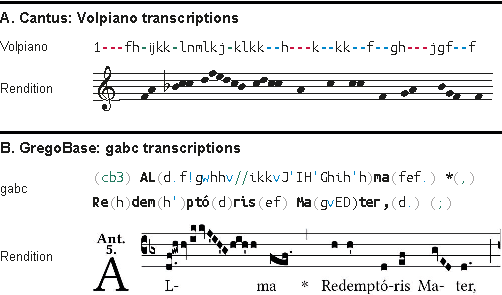
\includegraphics[width=\linewidth]{figures/fig01-volpiano-gabc.pdf}
    \caption{\normalfont
    %
    Two versions of \emph{Alma redemptoris mater}.
    (\textbf{\textsc{a}}) The CantusCorpus contains melodic transcriptions from medieval manuscripts notated in Volpiano: a simple five-line notation. (\textbf{\textsc{b}}) The Grego\-BaseCorpus contains scores from recent chant books in the gabc format, an elaborate format for four-line square notation.
    }%
    \label{fig:gabc-volpiano}
    \Description{Volpiano and gabc notation illustrated using two versions of Alma redemptoris mater.}
\end{figure}




\section{Corpora}
%————————————————


The first corpus we present, the CantusCorpus, is in essence a cleaned-up export of the Cantus database \cite{Cantus}.
This is an online index to the many medieval manuscripts kept in libraries across the world.
Currently it contains 497,071 chants; the database contains records for almost all, with information on where they are found in which manuscript, but also on things like their incipit, liturgical genre, feast, mode, and a \emph{Cantus ID} to be able to identify the same chants across manuscripts and databases.
For 63,628 chants (13\%) the melody has also been (partially) transcribed using \emph{Volpiano}.\footnote{%
    %————————
    Of the transcribed chants, 37\% contain fewer than 30 notes and are probably incipits.}
    %————————


Volpiano is a typeface that renders text as notes on five staff lines, and was specifically developed for notating plainchant.
Several conventions are commonly adhered to, such as the use of three, two and one hyphen(s) to indicate word, syllable and neume boundaries respectively (figure \ref{fig:gabc-volpiano}\textsc{a}).
This allows the music to be aligned to the manuscript text, which is transcribed separately.
Many of these conventions have been fixed in the elaborate transcription guidelines of the Cantus database and this is what we refer to as the \emph{(Cantus) Volpiano format.}
Such guidelines, and editorial reviews, ensure the high quality of the transcriptions \cite{Helsen2011}.


The Cantus database is easy to use for chant scholars, but not necessarily for computational purposes: 
it is continuously updated, which is actually inconvenient when replication is a concern.
We therefore scraped the database via its \textsc{api} and converted it to a set of clean \textsc{csv} files which we release as the CantusCorpus.
Releases are versioned as we plan to occasionally release newer versions.


Our second corpus, GregoBaseCorpus, again repackages and versions an existing database: GregoBase \cite{Gregobase}, which provides a complementary perspective on chant.
Whereas the Cantus database maps the complexity of medieval manuscripts in a simplified notation (Volpiano),
GregoBase consists of modern reinterpretations of the Gregorian repertoire: the one found in chant books like the \emph{Liber Usualis}.
Such books are indented for practical use and use the full scope of square notation, including things like breathing marks, different note shapes, rhythmic signs, and clef changes.

The GregoBase website currently hosts 9139 chant transcriptions from 29 books, including the complete \emph{Liber Usualis}.
The transcriptions are written in \emph{gabc} (figure \ref{fig:gabc-volpiano}\textsc{b}), a plain text format for square chant notation, developed 
for the typesetting system \emph{Gregorio}.
We converted the GregoBase database to a set of easy to use \textsc{csv} files, but also to separate gabc files that include metadata such as the mode, liturgical genre and all books a chant appears in.




\section{Chant21}\label{sec:chant21}
%———————————————————————————————————


\begin{figure}[t]
    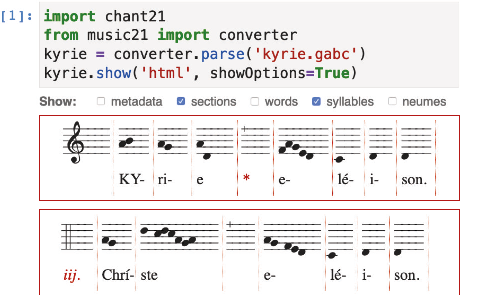
\includegraphics[width=\linewidth]{figures/fig02-chant21.pdf}
    \caption{\normalfont%
    \textbf{Chant21 in action.}
    %
    Chant21 improves the support for plainchant in Music21 with converters for gabc and Volpiano.
    It uses a chant representation that divides the chant in sections, words, syllables and neumes.
    This structure can be interactively explored in Jupyter notebooks.
    }%
    \label{fig:chant21-in-action}
    \Description{An screenshot of chant21 in action.}
\end{figure}


To make it easier to work with the two corpora we present the Python package chant21 which improves the support for gabc and Volpiano in music21 \cite{Cuthbert2010}, by now the go-to toolkit for symbolic computational musicology.
Chant21 consists of parsers for (1) gabc and (2) Volpiano; (3) a way to align text to music notated in  Volpiano; (4) a chant representation which retains the subdivision in sections, words, syllables and neumes; (5) a way to export this representation to \textsc{html}, which allows for fast visualization in Jupyter notebooks.


Writing parsers for the elaborate gabc syntax and the informal Volpiano guidelines is not straightforward.
After experimenting with custom parsers, we decided to specify the syntax of both formats as \emph{parser expression grammars} (\textsc{peg}s) \cite{Ford2004}.\footnote{%
    %————————
    This idea was borrowed from \texttt{gabc-parser}, but we had to completely rewrite the grammar as \texttt{gabc-parser} only implements the basic features of gabc and left many chants unparseable.}
    %————————
Specifying the syntax in a grammar makes it transparent and much easier to maintain.
\textsc{peg}s resemble context free grammars but use a deterministic choice operation to make parse trees unambiguous.
After specifying the grammar, we delegate the actual parsing to the \textsc{peg} parser \emph{Arpeggio} \cite{Dejanovic2016}.
The resulting parsers are reliable: their error rates are well under 1\% when evaluated on the CantusCorpus and Grego\-BaseCorpus and most failures are caused by syntax errors.


The parse trees of both gabc and Volpiano strings are then converted to music21 objects, but using a custom, hierarchical chant representation which groups the music in sections, words, syllables and neumes.
This structure can be useful in computational studies \cite{Cornelissen2020}, but is also needed to align Volpiano to the text.
The Cantus database has guidelines for full text transcriptions: how to for example mark section boundaries, or missing pitches.
We use another \textsc{peg}-based parser to parse the text, and then split all words in syllables using the Latin syllabifier from the \emph{Classical Language Toolkit} \cite{johnson2014}.
After all this, the text is divided in sections, words and syllables, which we match to their counterparts in the music.


Finally, inspired by the Cantus website, chant21 can export the hierarchical chant representation to \textsc{html}, using Volpiano to display the music.
This is particularly useful in Jupyter notebooks: it results in much faster typesetting and allows you to interactively explore the structure of the chant.
After installing Volpiano and running \texttt{pip install chant21}, chant21 is ready to be used (figure \ref{fig:chant21-in-action}).




\section{Case study I: the melodic arch}
%———————————————————————————————————————

\begin{figure}[t]
    \centering
    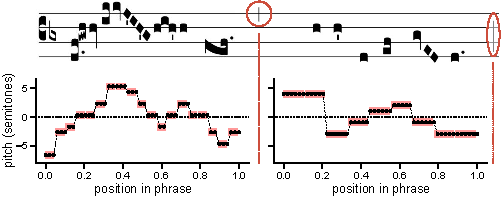
\includegraphics[width=\linewidth]{figures/fig03-contour-representation}
    \caption{\normalfont%
    \textbf{Contour representation.}
    %
    Contours consist of 50 pitches, sampled after normalizing the phrase duration and transposing the phrase by its mean pitch. This is illustrated the first two phrases of the antiphon \emph{Alma mater redemptoris}. The plots below the score shows the contours in black over a red piano roll.
    }%
    \label{fig:contour-representation}
    \Description{Illustration of the representation used in the first case study.}
\end{figure}

\begin{figure}[t]
  \centering
  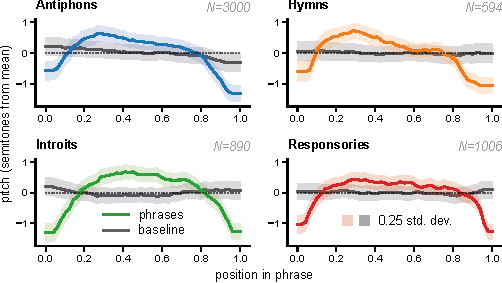
\includegraphics[width=\linewidth]{figures/fig04-average-phrase-contours.pdf}
  \caption{\normalfont%
    \textbf{Average phrase contours.} 
    %
    The melodic arch hypothesis seems to hold in Gregorian chant.
    Averaging all phrase contours results in arch-shaped contours (coloured), whereas averaging random segments (grey) yields more or less flat contours.
    This is illustrated for four chant genres.
    }%
    \label{fig:average-phrase-contours}
    \Description{Average phrase contours of four chant genres.}
\end{figure}


To illustrate the usefulness of the presented corpora and software, we discuss two case studies.\footnote{%
    %————————
    \label{fn:repository}
    For the data and code of the case studies, see \href{https://github.com/bacor/DLfM2020}{github.com/bacor/DLfM2020}}
    %————————
The first concerns the \emph{melodic arch hypothesis}: the claim that the pitch contour of musical phrases across cultures tend to be arch-shaped.
David Huron \cite{Huron1996} was the first to present quantitative support for this phenomenon, based on an analysis of 6000, mostly German folksongs from \emph{Essen}.
Later studies confirmed the hypothesis in the 2000 Chinese folksongs that were later added to \emph{Essen} \cite{Tierney2011}, and a small global sample of 35 recordings from the Garland Encyclopedia \cite{Savage2017a}.


It has been suggested that the melodic arch is the result of general motor constraints \cite{Tierney2011}.
Those make it easier to produce rising pitch contours at the start of a phrase, when the pressure beneath the vocal folds is rising, and falling contours when the pressure drops towards the end.
These constraints could imply a weak tendency for phrases to be arch-shaped (or descending) \emph{on average}, even though individual phrases can take many shapes.


We analyze if these findings extend to Gregorian chant and focus on the \emph{Liber Usualis} from the GregoBaseCorpus (v0.4).
We extracted phrases using the explicit breathing marks (\emph{pausas}) in chant notation.
As rhythmic interpretations of chant vary, we assigned all notes in chants equal duration.
We removed duplicate phrases and phrases with fewer than 4 notes, and then randomly sample 3000 phrases per chant genre.
Finally, we normalized all phrases to have duration 1 and mean pitch 0, and sampled 50 equally spaced pitches from the resulting contour \cite{Tierney2011,Savage2017a}, as illustrated in figure \ref{fig:contour-representation}.


We average the 3000 normalized contours of a given genre and compare this to the following random baseline.
We randomly segment every chant by successively sampling segment lengths from a Poisson distribution approximating the actual phrase lengths.
The first and final (random) segments of each chant are omitted.
This results in a set of random segments whose lengths are similar to actual phrases, but whose boundaries are unlikely to overlap with actual phrase  boundaries.
This keeps the melody intact and only shifts phrase boundaries---rather than shuffling all pitches \cite{Savage2017a}.


Figure \ref{fig:average-phrase-contours} shows the average phrase contours (coloured) compared to the average random segments (grey) for four chant genres.
Whereas the actual phrases are clearly arch-shaped on average, the baseline is pretty much flat.
The overall size of the arch is small (around 2 semitones), but similar to earlier findings \cite{Tierney2011,Savage2017a}.
The average contours appear to differ across genres, but it requires further analyses to see if these differences are significant.
The comparison with the random baseline does however make clear that phrase boundaries have a noticeable and consistent effect on the shape of phrase contours.
In sum, these results from this corpus of plainchant are consistent with the melodic arch hypothesis.




\section{Case study II: differentiæ}
%———————————————————————————————————


Our second case study revisits a particular problem in chant scholarship which also figured in a recent edition of this conference: the relation between so-called \emph{differentiæ} and antiphon openings \cite{Shaw2018}.
Every week, monks would sing a cycle of 150 psalms to melodic formulae known as psalm tones.
An antiphon was sung before the psalm, and repeated afterwards.
The \emph{differentiæ} is the very end of the psalm, always set to the words \emph{sæculorum amen} (abbreviated as \emph{euouae}) and sung directly before the repetition of the antiphon.
The order, in short, was always antiphon--psalm-- differentia--antiphon.
A question dividing chant scholars is whether there is a systematic relation between differentiæ and antiphon openings: do certain psalm endings usually imply certain antiphon openings?

Rebecca Shaw \cite{Shaw2018} conducted the first large-scale data analysis and suggests that there is indeed a systematic connection for mode 1.
Using chant21 we can extend this to all eight modes by visualizing the connections directly.
We selected all 7102 antiphons from the CantusCorpus (v0.1) that had a complete Volpiano transcription, lyrics ending on variants of \emph{aeouae}, and a `simple' mode (e.g., not transposed).
We extract the last 6 pitches of the differentia and concatenate the first 6 notes of the antiphon to obtain the \emph{(differentia--antiphon) connections}.
We transpose all connections so that the final has pitch 0.


\begin{figure}[t]
  \centering
  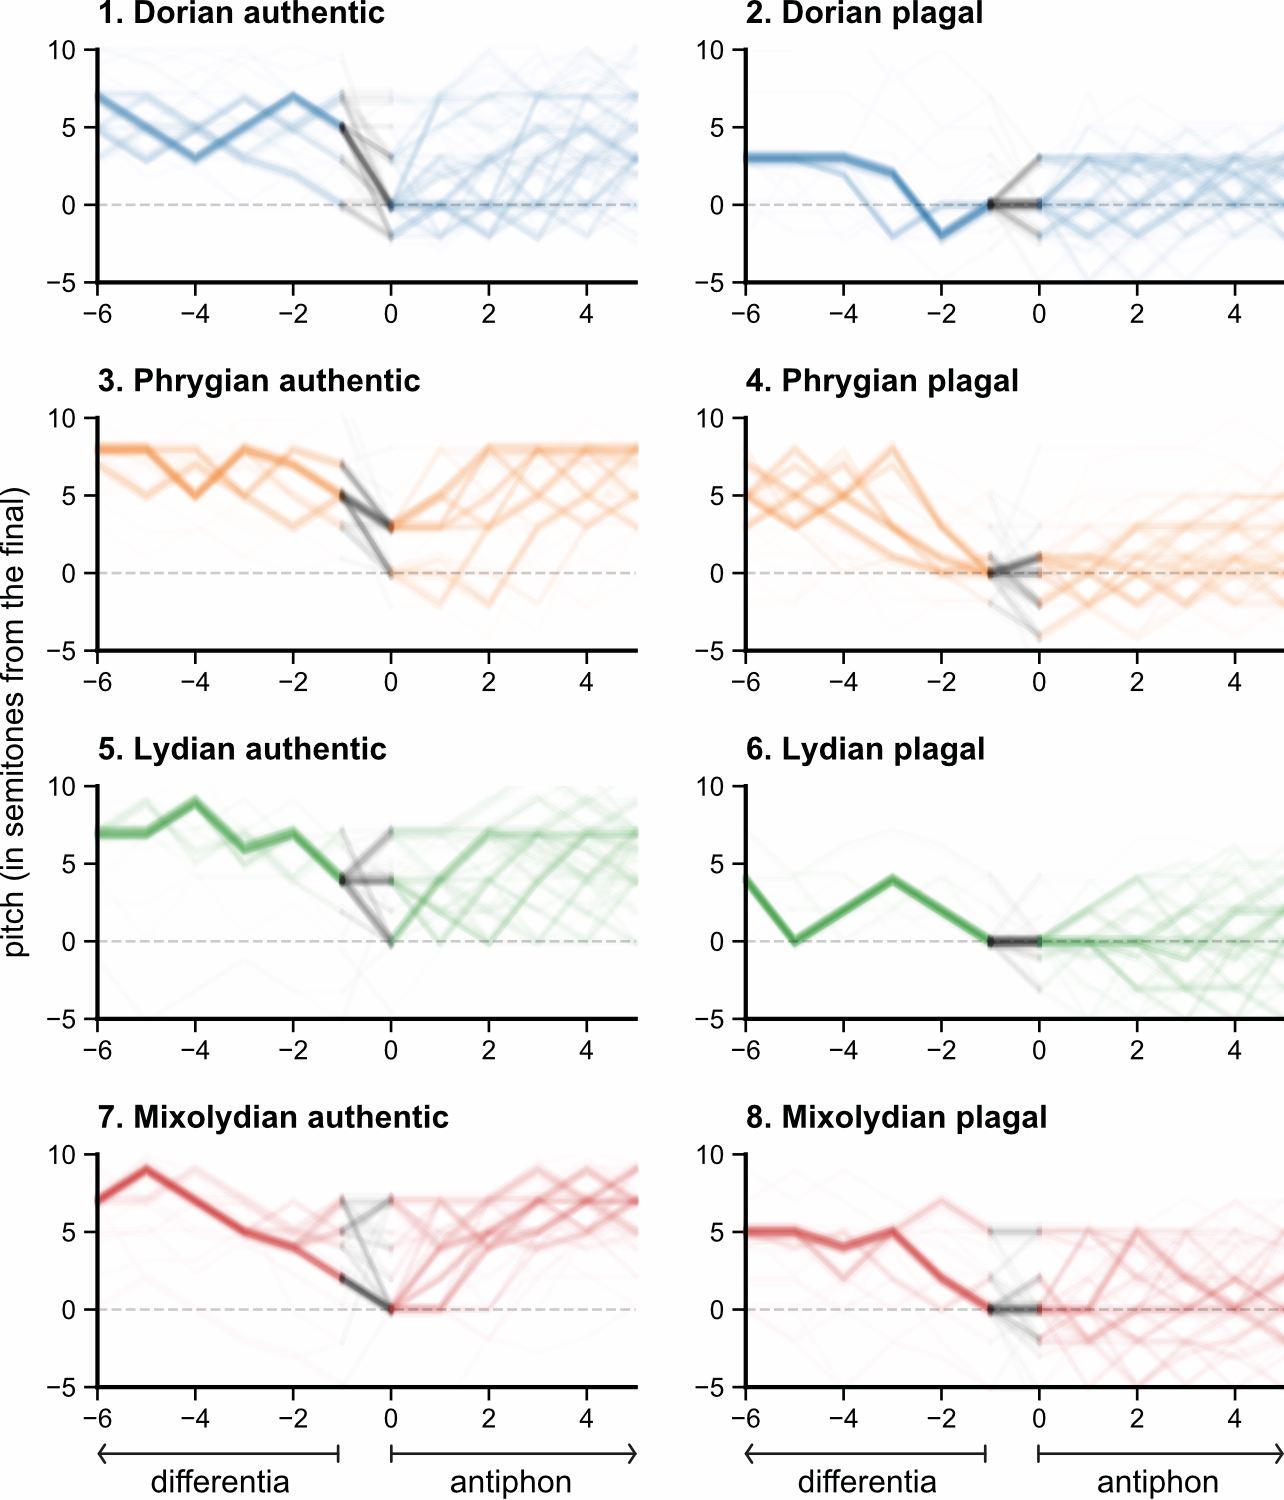
\includegraphics[width=\linewidth]{figures/fig05-connections.png}
  \caption{\normalfont%
    \textbf{Differentia-antiphon connections} in all modes.
    Each line represents the last 6 notes of the differentia (coloured), followed by the return to the antiphon (black), and 5 more notes of the antiphon (coloured).
    We sample and show 200 connections per mode, jittered vertically to reveal clusters of overlapping contours.
    }%
    \label{fig:connections}
    \Description{Visualization of differentia-antiphon connections in all modes.}
\end{figure}


Figure \ref{fig:connections} shows the connections for all modes.
The systematicity seems to differ between modes.
For example, mode 6 exhibits a very systematic connection: only one differentia is really ever used, and this virtually always leads to the same starting pitch of the antiphon (the final, \textsc{f}).
Mode 5, on the other hand, also uses mostly one differentia, but this leads to three possible antiphon openings.
This is certainly less systematic, but more predictable than a random transition.


This suggests a way to quantify the systematicity.
For a given mode, consider all the segments $s_{-3:0} = (n_{-3}, n_{-2}, n_{-1}, n_0)$ spanning the last 3 notes of the differentia and the first of the antiphon.
If we compute the relative frequencies $p(s_{-3:0})$ of all those segments, we find that in mode 6 only one segment is very frequent, where in, say, mode 4 multiple segments are relatively frequent.
One way to quantify this is using the \emph{entropy} $H(p(s_{-3:0}))$ or $H_{-3:0}$ for short, of those relative frequencies: this is a measure of the unpredictability of the chant in the segment from position $-3$ to position $0$.
This is what we show in figure \ref{fig:entropy}\textsc{b}.
We can repeat this starting at different positions $t$ in the chant, and compute the entropy $H_{t:t+3}$ in all windows of four notes.
We did this in figure \ref{fig:entropy}\textsc{a}; it shows how unpredictable different parts of the chant are.
It is immediately clear that the more formulaic differentia ($t \le -4$) are indeed more predictable than antiphons ($t\ge 0$).
But we also see that the moment we return to the antiphon, the entropy increases: $H_{-4:-1}<H_{-3:0}$.
This suggests that across modes, differentia--antiphon connections are less predictable than differentiæ, but more predictable than antiphon openings.


\begin{figure}[t]
  \centering
  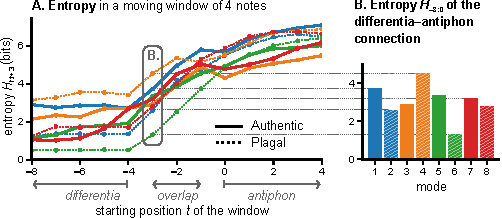
\includegraphics[width=\linewidth]{figures/fig06-entropy.pdf}
  \caption{\normalfont%
    \textbf{Entropy of the chant.}
    %
    (\textbf{\textsc{a}}) We move a sliding window of 4 notes across the chant and estimate the unpredictability in the window using the entropy $H_{t:t+3}$ (details in main text).
    This shows that differentiæ ($t\le -4$) are more predictable than antiphons ($t \ge 0$).
    (\textbf{\textsc{b}}) Highlights the window containing the last 3 notes of the differentia and the first note of the antiphon, showing for example that the connection in mode 6 is more predictable than in mode 4.
    }%
    \label{fig:entropy}
    \Description{Entropy of the differentia-antiphon connection in all modes.}
\end{figure}




\section{Conclusions}
%————————————————————


We have presented two large corpora of Christian plainchant, the Python library chant21 which allows them to be used in music21, and two case studies.
First, we showed that phrase contours in the GregoBaseCorpus confirm the melodic arch hypothesis.
Second, we show that the connection between differentiæ and antiphon openings is less predictable than the connection between notes within differentiæ, but more predictable than  within antiphons.
Moreover, the relation clearly differs across modes.
Both case studies only scratch the surface, and raise further questions.
We hope that this work will inspire more computational studies of plainchant, and broaden the traditions studied by computational musicologists.

%%
\pagebreak

\bibliographystyle{ACM-Reference-Format}
\bibliography{bibliography}

\end{document}
\endinput